% https://www.naept.com/en/blog/validation-plan-check-your-product-meets-the-customer-needs-part-one/
\setchapterpreamble[u]{\margintoc}
\chapter{Validation Plan\\Check your product meets the customer needs}
\label{sec:ValidationPlan}

We’ll see how to build a validation plan ensuring your product is matching all your customer’s requests.

\section{What is it used for?}

The more complex products you create, the more difficult it is to check they fit all the customer’s specifications. In the chapter ~\ref{TraceabilityMatrices}, we talked about the traceability matrices, the dependency connections between the customer’s need and your product’s features can be numerous! And when you deliver your product (or your service), you have to be sure that all those features are correctly working.

Besides, sometimes a new feature request happens and challenges all the work previously done: “Now the car must carry 7 people, not just 5”. “OK so the car must be longer, the engine stronger…”. Those evolutions shall not alter what was correctly working earlier. To validate this point we have to perform “regression tests”.

This is why creating a list of test checking that each and every feature works correctly with the other is crucial. Such a list is what we call a validation plan.

\section{What does it look like?}
Depending on the complexity of you project, the way you describe your tests can takes different shapes: from a very light one to the most bullet-proof. We have identified 3 ways:

\subsection{1. In the same document than your product’s specifications}

\begin{figure}[h]
    \centering
    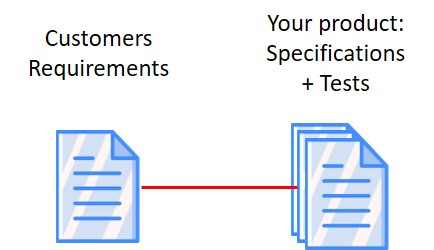
\includegraphics[]{1-in-the-same-document.jpg}
    \caption{The product specifications and tests are in the same document}
    \label{fig:SameDocument}
\end{figure}

Your customer has described his need in a requirements document. You reply to it in a specifications document where you explain all the features of you future product. Each of those features is followed by a corresponding test with a status checkbox telling if it is OK or not.

Like this you reduce the number of documents by gathering everything in one.

But if the project grows and the product requires more complex features, you may want to test several of them at once if you can. This format doesn’t allow this kind of test management: you cannot “factorize” the tests and therefore you may have redundancies. Which is not very efficient.

\subsection{2. List the tests in a separate document}

\begin{figure}[h]
    \centering
    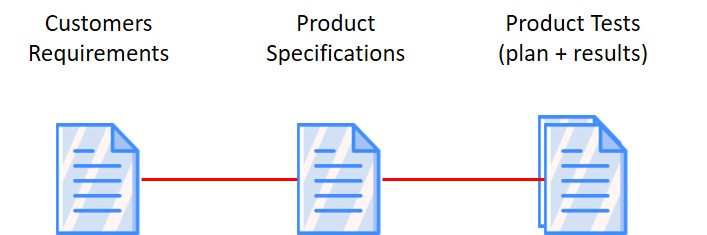
\includegraphics[]{2-in-two-document.jpg}
    \caption{Tests in their own document}
    \label{fig:TwoDocument}
\end{figure}

Your customer has described his needs in a requirements document. You reply to it in a specifications document. And you describe the tests on those specifications in a third document. Each test can have specific fields to precise details on the results (measured values, expected results, status, comments\dots).

The benefit is that you can now factorize the tests: in one bigger test you can check the validity of several specifications at once and reduce the time spent on this activity.

The drawback is now you have to keep track of the links between the specifications and their tests. But it is easy to do so with traceability matrices.

Now, a new hidden problematic comes out. It only occurs if you have to perform your tests several times. Let’s take a concrete example. Imagine you are a reusable anti-COVID masks manufacturer (not the disposable ones). So you deliver lots of masks, all the same, and you have to test each and everyone of them before to put them on the market. For each mask you have to duplicate the test document to perform the campaign, and to fill it with the mask tests results but the test descriptions are exactly the same. That makes a lot of redundancy between the 2 documents. Let’s see how to optimize this…

\subsection{3. Cut the test document in 2: the procedures and the results}

\begin{figure}[h]
    \centering
    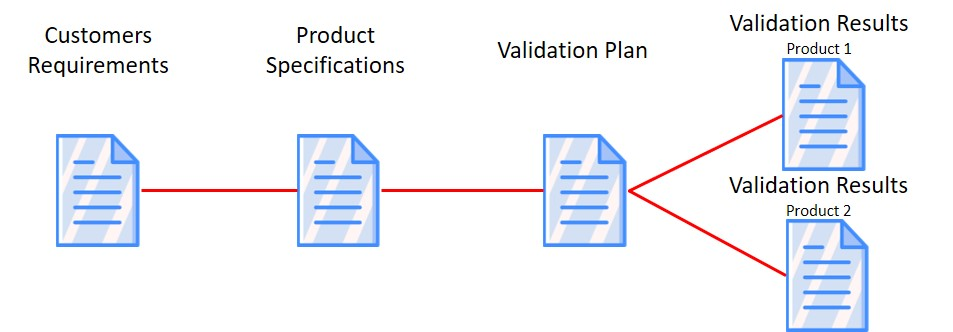
\includegraphics[]{3-in-three-documents.jpg}
    \caption{Test procedures and results in 2 documents}
    \label{fig:ThreeDocument}
\end{figure}

Here is the best way to do, from our point of view:

\begin{itemize}
    \item The tests procedures are detailed in a first document: the validation plan
    \item All the results for the same product are gathered in its own document: the validation results
\end{itemize}

OK the obvious drawback is the multiplication of the documents. From “one doc to rule them all” we go to at least 3 (specifications, validation plan and validation results) and more if you deliver several identical products. And off-course you have to manage a traceability matrix for each document relation (red link).

BUT,

it is the best way for us because of the following reasons:

\begin{itemize}
    \item Each document deals with only one aspect of the project: specifications design the solution, validation plan builds the tests, validation results report the status on the product.
    \item Each document is therefore shorter and so easier to maintain up to date.
    \item Consequently, each document can evolve independently from the other one. And if there is an impact, the traceability matrices will tell you exactly where.
\end{itemize}

In the following sections, we will explain the organizations of the validation plan and results in two separated document. But even if they are merged it works the same.

\section{The procedures}
In the validation plan you will define all the procedures for the required tests to validate that your product correctly matches its specifications.

The validation plan will contain enough tests if and only if all of the specifications are covered by one test at least. Although it doesn’t mean there should be one test for each specification. And this is one major benefit of the validation plan, you can do:

\begin{itemize}
    \item one test for one specification
    \item one test for several specifications at once
    \item several tests to check only one complex specification
\end{itemize}

That’s why traceability matrices are very useful! By tracking all those relations they ensure at least one test covers each specification. If it is not the case, you know you need more tests and what to do them on.

\section{How to structure a test procedure?}
A test procedure is divided in two parts:

\begin{itemize}
    \item The test identification
    \item The test steps
\end{itemize}

\subsection{The test identification}
This identification gathers several metadata about the test itself. Here are the most essential ones.

\subsubsection{A unique reference}
This reference allows to identify instantly the test without any doubt. It will be useful in the traceability matrices. It can be followed by a revision number to track the evolutions on the test: each modification of the text increases its revision number.

Ex.: NPT\_ProjectVehicule\_VP\_0301.1

\subsubsection{A title}
It is required to have a title telling in a few words the purpose of the test. It is essential to quickly know what the test is about, and refer it easily in a conversation with coworkers for example.

Ex.: “Check the front light”

\subsubsection{A description}
You explain here the purpose of the test. What is it doing, why and maybe how the test is supposed to end. Sometimes the person writing the test (the author) is not the same person to perform it (the operator). The description will give the operator some details about the context and what he should expect.

Ex.: “The purpose of this test is to check the front light of the car are correctly working and manageable from the pilot seat.”

\subsubsection{Initial conditions}
This is a very important item! Setting initial conditions allows to sequence your validation plan.

Some tests can require to be done within specific conditions. They may be possible only under certain circumstances.

For example, a test might be so long, it would be easier to cut it in half. Therefore the second part can only be performed if the first part is OK. So the success of part one is the “initial condition” for part two.

Another example, several tests can have their first steps in common. You may want to gather those redundant steps in a dedicated test to do it just once and cut this part from the other tests. You will gain some precious time and those tests require to have this initial condition (the first steps) to be previously done.

Ex.: This test requires the followings tests to be passing:

NPT\_ProjectVehicule\_VP\_0230.1 : Check the car start-up\\
NPT\_ProjectVehicule\_VP\_0254.1 : Check the car’s wiring

\subsubsection{The traceability}
With this item, you list all the specifications this test validates.

So the compilation of all the tests traceabilities tells you exactly which specifications are tested and which are not. So you can calculate the coverage of your validation plan, you know if it is complet or needs some more tests.

Ex.: Coverage:
\begin{itemize}
    \item NPT\_ProjectVehicule\_SPEC\_0058.1
    \item NPT\_ProjectVehicule\_SPEC\_0022.1
    \item NPT\_ProjectVehicule\_SPEC\_0137.1
    \item NPT\_ProjectVehicule\_SPEC\_0796.1
\end{itemize}

\subsubsection{Other possible items}
Here are some items you can add to the test identifications:

\begin{itemize}
    \item \textbf{The kind of test}: tests can be categorized depending on the way to perform them. There are inspection test where you just have to visually check the presence of an element. There are the certification tests where you need to have a certificate from the supplier officially telling you the device is working. The demonstration tests that require to manipulate the device to obtain the expected behavior…
    \item \textbf{The gravity}: some tests may be more important than other. If a low gravity test is not ok, may be it’s not a big deal and the device is still good enough to be delivered. By giving gravity indication on tests, you can sort them to prioritize the most important ones.
\end{itemize}

\subsection{The test steps}
This is here we go deep into the test procedure, step by step. The procedure is basically a table where each line is a test step. I strongly recommend to explicitly sequence the procedure step by step. The best procedure is the one that can be performed by a total stranger to the project as everything is completely detailed.

This exhaustiveness principle brings several benefits:

\begin{enumerate}
    \item Having a crystal clear procedure allows the test operator to focus on the unit under test and how it reacts. But if he has to question the procedure or to guess if he understands it well enough, he will also question the results he observes. He won’t know if he’s doing right or if he misses something if the procedure allows to doubt.
    \item The procedure can be performed by a stranger and this stranger won’t be biased. Such an operator is better at finding bugs or fault (See Fix your product issue with a problem report). Besides if the procedure can be performed by a stranger, and if you need more people to do the tests because of a deadline, anyone can help you!
\end{enumerate}

Let’s see the different columns we suggest you to put in your test procedure:

\subsubsection{Step number}
This number allows precisely identifying the step in a comment, a potential exchange or even in another step to do a loop in the procedure : “If it is NOK, go back to step \#6“.

\subsubsection{Expected result}
This item is not systematic. If the action doesn’t expect a specific one, do not tell one. On the other hand, if there is one and if it will decide the status of the test, therefore you need to be very specific too:

\begin{itemize}
    \item If what is expected is a behavior, then be very detailed about it without any possible doubt. We don’t want the operator to miss it
    \item If a measure is expected: a number of items, a voltage, a length… Then tell the expected measure’s value, unit and tolerance.\\Example: you expect a board to be 2 meters long more or less 1 centimeter (or 0,01 m).\\If the measured length is 2,005 m then the test is OK.
\end{itemize}

\subsubsection{Some other attributes}
Here are some more attributes to add to the procedure table:

\begin{itemize}
    \item \textbf{Traceability} : you can tell for each step the specification it validates. You may just fill it for the steps with an expected result and not for the others. It allows to rapidly see which part of the procedure is critical but it can be redundant with the traceability given in the test identification.
    \item \textbf{How to manage NOK steps}: when a step is OK, we implicitly go for the next one. But what if the step is not OK (NOK)? Should we leave the UUT in this state? You may have to properly shut it down. So you could describe in a new column what to do if the step is NOK. You can write a “shut down procedure” in the validation plan, and you can refer to this procedure in the step in the case where the step is NOK.
\end{itemize}


Et Voilà for the structuring of the test procedures. Don’t forget to add the traceability matrices at the end of the validation plan to keep track of the coverage.

\section{The validation results}
It’s like the little brother of the test procedures. This report document contains all the results of all the tests for one sample of the product to be delivered. And this time, for each procedure there is only one test report. This will ease the traceability matrix between the validation plan and the validation results as their relation is 1:1.

In the previous article, we saw that the benefits of separating the procedures from the results in 2 different documents is to be able to perform the validation plan on several identical products. So the validation results are belonging to one and only one copy of the product. So this is the first thing to do: uniquely identify the copy of the product to be tested.

\subsection{Identifying the UUT}
UUT or Unit Under Test, is the generic name given to the product that is tested. So now I’ll refer to it as the UUT.

In the very beginning of the result document, we will dedicate a paragraph to identify the UUT. The purpose is to associate the result document to only one copy of the product and be sure not to mix it with another copy. Though the serial number is one piece of data to identify a product, here are a list of information useful to complete the identification:

\begin{itemize}
    \item Model number or name. Ex.: “iPhone”
    \item Revision number. Ex.: “12”
    \item Serial number. Ex.: “98765431”
    \item Date of manufacture. Ex.: “October 2020”
\end{itemize}

With all those element : “iPhone 12, S/N: 98765431, October 2020”, we are very sure there is not another copy of the product with the same attributes.
In the eventuality that this precise product is malfunctioning and the customer returns it, it will be easy the find the corresponding validation results to check if all the tests had been correctly done.

To have a better overview, we can define a global validation status telling you at once if the product is OK or not. This status is the compilation of all the test results statuses. This global status can obviously be filled out once all the validation plan tests have been performed at least once. And then, for more details you can go for the procedure result you want.

\subsection{How to structure the results for each procedures?}
Now that the UUT is clearly identified, let’s see the reports. Just like the procedures in the validation plan, they are divided in 2 sections:

\begin{itemize}
    \item The test results identification
    \item The results step by step
\end{itemize}

\subsubsection{The test results identification}

\paragraph{The reference}
Remember, to reduce the size of the report, we decided not to put the procedures in it, so to understand the results we recall the reference of the test procedure they are about.

\paragraph{The title}
For comfort, we repeat the title of the procedure. It easier when you browse the results to look for an understandable title than a cryptic reference.

(So now you think: what’s the purpose of the reference then? Well, when you need to refer to the test in another document, you will prefer a short reference to a long explicit title.)

\paragraph{The timestamp}
We tell the date and time of the moment the results has been obtained / the test sequence has been performed. This would be very useful in case of a future issue with this product. We will be able to cross those data with some other data, like log files or automatic reports from other tools, if we need to investigate.

\paragraph{Identification of the test operator}
When several people have to perform the tests or when the operator is different from the developer, it is useful to identify them.

In case of a failed test, the person in charge of fixing the problem may need some more information and would question the operator (See Problem Report, Fix your product issue).

\paragraph{The test status}
This is the most important piece of information. It is the compilation of all the step statuses. It can tell in a glimpse if the UUT has passed the procedure or not. If not, we can go look for the test comments or for the specific failed step.

Commonly, for a test to be fully “OK”, all the steps must be successfully passed.
On the other side, for the test to fail, it only requires one step to be not OK!

But a failed test doesn’t necessarily imply the UUT is deficient. Maybe the procedure isn’t mature enough and needs to be updated.

\paragraph{Comment}
It allows the operator to add some precision elements about the course of the procedure. He can write down observations and details about what happened when the test failed for example.

\paragraph{Those attributes we do not repeat from the procedure}
As the relation between the report and the procedure are 1:1, there is no need to repeat the test description, the traceability or the initial conditions. They would only make the report heavier and its update more difficult (that’s why we cut it in half).

\subsubsection{The results step by step}
\paragraph{Step number}
This is the same number we have on the procedure to link the result to the corresponding step.

\paragraph{Measure}
This column allows to enter a measure eventually required by the step. If the step doesn’t ask for it, leave a blank case.

\paragraph{Status}
You can set a status for each step telling if it has been passed successfully or not:

\begin{itemize}
    \item \textbf{Done} / \textbf{OK}: for a step that doesn’t expect any specific result. Therefore you simply check it was done, so a checkbox could be enough.
    \item \textbf{OK}: the step required a specific result that perfectly happened.
    \item \textbf{NOK} (for Not OK) / \textbf{Failed} : the step required a specific result that didn’t happen as expected.
\end{itemize}

\paragraph{Step comment}
Having a comment column to add details to a specific test in case of a failure can be really helpful to investigate the problem.

\paragraph{Some other possible attributes}
\textbf{Action}: When a step fails, it might be because of an issue with the UUT and a problem report should be initiated. Or it may be because of the test procedure that must be updated, in this case a reading sheet shall gather the remarks about the procedure. Therefore the Action field is used to give the reference of such file that will document the fixing action. So you can track all the strategy and all the modifications upon the procedure.

This concludes our proposition for a better structure of the product validation plan. Now I’d like to draw your attention on one last thing to reach a greater quality level.

\section{The importance for the author, the maker and the test operator to be 3 different people}
This measure can look expensive at first, but if you have to perform tests at great scale, it can significantly reduce the bias and increase the quality.

First of all, the author is the collaborator writing the tests procedures. This is the person who has designed them.
The maker is the person who has built the product or realized the service. He has shaped what was designed.
And finally the test operator is the one performing the tests (designed by the author) onto the product (built by the maker).

In a perfect world (and such a world is very expensive, we all agree), all three of them are different people. But in practice, because of the budget or the planning, all of them might be merged into the same person. This person knows perfectly its product. So when she tests it, she can unconsciously but slightly adapt the procedure to make it pass. Or worse, she will be willing to make it pass. But this is precisely the point of the test: finding the failures to fix them before delivery.
In the other way, a different person as the test operator will have no idea on how a product works. So he will methodically follow the procedure and be very good at finding those failures (from the product or from the procedure).

That is why it is very efficient to separate those 3 steps in the development of a product : design, realization and tests. It will reduce the risks of human bias or conflict of interest. But they need to work very closely to avoid inertia. A project management is always a clever compromise between quality, cost and delays.

(In the end, it is one more reason for identifying the person performing the test in the report!)

\section{Conclusion}
As we saw it in this article, building and performing a test plan is a real project within a project. But it is essential to ensure a high quality product.

It would be easy to believe that the multiple documents, detailed here, make the project management heavier. But at the end of the day, they don’t. Yes they require a little more time at the beginning of the project but they induce more flexibility and therefore a better resilience. Ok there are more documents but they are shorter and easier to maintain.

If the customer’s requirements evolve, you’ll only have surgical modifications to make which will be pointed out by the traceability matrices.
